\documentclass[table]{beamer}
%[]中可以使用handout、trancompress等参数

%指定beamer的模式与主题
\mode<presentation>
{
  \usetheme{Madrid}
%\usetheme{Boadilla}
%\usecolortheme{default}
%\usecolortheme{orchid}
%\usecolortheme{whale}
%\usefonttheme{professionalfonts}
}

%\usetheme{Madrid}
%这里还可以选择别的主题:Bergen, Boadilla, Madrid, AnnArbor, CambridgeUS, Pittsburgh, Rochester, Warsaw, ...
%有导航栏的Antibes, JuanLesPins, Montpellier, ...
%有内容的Berkeley, PaloAlto, Goettingen, Marburg, Hannover, ...
%有最小导航栏的Berlin, Ilmenau, Dresden, Darmstadt, Frankfurt, Singapore, Szeged, ...
%有章和节表单的Copenhagen, Luebeck, Malmoe, Warsaw, ...

%\usecolortheme{default}
%设置内部颜色主题(这些主题一般改变block里的颜色);这个主题一般选择动物来命名
%这里还可以选择别的颜色主题,如默认的和有特别目的的颜色主题default,structure,sidebartab,全颜色主题albatross,beetle,crane,dove,fly,seagull,wolverine,beaver

%\usecolortheme{orchid}
%设置外部颜色主题(这些主题一般改变title里的颜色);这个主题一般选择植物来命名
%这里还可以选择别的颜色主题,如默认的和有特别目的的颜色主题lily,orchid,rose

%\usecolortheme{whale}
%设置字体主题;这个主题一般选择海洋动物来命名
%这里还可以选择别的颜色主题,如默认的和有特别目的的颜色主题whale,seahorse,dolphin

%\usefonttheme{professionalfonts}
%类似的还可以定义structurebold,structuresmallcapsserif,professionalfonts


% 控制 beamer 的风格,可以根据自己的爱好修改
%\usepackage{beamerthemesplit} %使用 split 风格
%\usepackage{beamerthemeshadow} %使用 shadow 风格
%\usepackage[width=2cm,dark,tab]{beamerthemesidebar}
\usepackage{booktabs}
\usepackage{caption}
\usepackage{subcaption}
\usepackage{tikz}

\usepackage{xcolor}
\usepackage{graphicx}
\usepackage{ulem}
\usetikzlibrary{decorations.pathmorphing,decorations.pathreplacing,calc}


%\textcolor{red/blue/green/black/white/cyan/magenta/yellow}{text}
%颜色设置
\usepackage{colortbl}
\definecolor{mygray}{gray}{.9}
\definecolor{mypink}{rgb}{.99,.91,.95}
\definecolor{mycyan}{cmyk}{.3,0,0,0}

% 设定英文字体
\usepackage{fontspec}
\setmainfont{Times New Roman}
\setsansfont{Arial}
\setmonofont{Source Code Pro}

% 设定中文字体
\usepackage[BoldFont,SlantFont,CJKchecksingle,CJKnumber]{xeCJK}
%\setCJKmainfont[BoldFont={Adobe Heiti Std},ItalicFont={Adobe Kaiti Std}]{Adobe Song Std}
\setCJKmainfont[BoldFont={Adobe Heiti Std},ItalicFont={Adobe Kaiti Std}]{WenQuanYi Micro Hei}
\setCJKsansfont{Adobe Heiti Std}
\setCJKmonofont{Adobe Fangsong Std}
\punctstyle{hangmobanjiao}

\defaultfontfeatures{Mapping=tex-text}
\usepackage{xunicode}
\usepackage{xltxtra}

\XeTeXlinebreaklocale "zh"
\XeTeXlinebreakskip = 0pt plus 1pt minus 0.1pt

\usepackage{setspace}
\usepackage{colortbl,xcolor}
\usepackage{hyperref}
%\hypersetup{xetex,bookmarksnumbered=true,bookmarksopen=true,pdfborder=1,breaklinks,colorlinks,linkcolor=blue,filecolor=black,urlcolor=cyan,citecolor=green}
\hypersetup{xetex,bookmarksnumbered=true,bookmarksopen=true,pdfborder=1,breaklinks,colorlinks,linkcolor=cyan,filecolor=black,urlcolor=blue,citecolor=green}

% 插入图片
\usepackage{graphicx}
% 指定存储图片的路径(当前目录下的figures文件夹)
\graphicspath{{figures/}}

% 可能用到的包
\usepackage{amsmath,amssymb}
\usepackage{multimedia}
\usepackage{multicol}

% 定义一些自选的模板,包括背景、图标、导航条和页脚等,修改要慎重
% 设置背景渐变由10%的红变成10%的结构颜色
%\beamertemplateshadingbackground{red!10}{structure!10}
%\beamertemplatesolidbackgroundcolor{white!90!blue}
% 使所有隐藏的文本完全透明、动态,而且动态的范围很小
\beamertemplatetransparentcovereddynamic
% 使itemize环境中变成小球,这是一种视觉效果
\beamertemplateballitem
% 为所有已编号的部分设置一个章节目录,并且编号显示成小球
\beamertemplatenumberedballsectiontoc
% 将每一页的要素的要素名设成加粗字体
\beamertemplateboldpartpage

% item逐步显示时,使已经出现的item、正在显示的item、将要出现的item呈现不同颜色
\def\hilite<#1>{
 \temporal<#1>{\color{gray}}{\color{blue}}
    {\color{blue!25}}
}

% 自定义彩色块状结构的颜色
\setbeamercolor{bgcolor}{fg=yellow,bg=cyan}

% 在表格、图片等得标题中显示编号
%\setbeamertemplate{caption}[numbered]

% 打开PDF后直接全屏
\hypersetup{pdfpagemode={FullScreen}}


% 使用 \part,\section,\subsection 等命令组织文档结构
% 使用 \frame 命令制作幻灯片

\begin{document}

\logo{
\includegraphics[height=0.09\textwidth]{gm.jpg}}
\title[价格生成机制]{交易规则与价格生成机制}
\author[李波文]{李波文}
\institute[GOLDMINER]{掘金量化交易平台}
\date{\today}

% 定义目录页
\AtBeginPart{
  \frame{
    \frametitle{\partpage}
    \begin{multicols}{2}
% 如果目录过长,可以打开这个选项分两栏显示
      \tableofcontents
% 使用这个命令自动生成目录
    \end{multicols}
  }  
}

% 在每个Section前都会加入的Frame
\AtBeginSection[]
{
  \begin{frame}<beamer>
    \frametitle{提纲}
	\setcounter{tocdepth}{2}
    \tableofcontents[currentsection,currentsubsection]
  \end{frame}
}
% 在每个Subsection前都会加入的Frame
\AtBeginSubsection[]
{
  \begin{frame}<beamer>
%\begin{frame}<handout:0>
% handout:0 表示只在手稿中出现
    \frametitle{提纲}
	\setcounter{tocdepth}{2}
    \tableofcontents[currentsection,currentsubsection]
% 显示在目录中加亮的当前章节
  \end{frame}
}

\begin{frame}
  \titlepage
\end{frame}

\begin{frame}[plain]
  \frametitle{提纲}
  \setcounter{tocdepth}{2}
  \tableofcontents
\end{frame}

\section{Trick: Spoofing}

\begin{frame}{Spoofing}
  \begin{columns}
    \column{6cm}
\begin{table}
  \centering
    \begin{subtable}[b]{0.4\textwidth}
    \resizebox{\textwidth}{!}{
      \setlength{\arrayrulewidth}{2pt}
      \arrayrulecolor{orange}
      \begin{tabular}{|c|c|}
        \arrayrulecolor{orange}\hline
        \multicolumn{1}{>{\columncolor{cyan}}c|}{\color{white}\textsf{Offer Price}} &  \multicolumn{1}{>{\columncolor{cyan}}c}{\color{white}\textsf{Offer Quantity}}\\ 
        \arrayrulecolor{orange}\hline
        \rowcolor{mycyan}
        {} & {} \\
        \arrayrulecolor{orange}\hline
        \rowcolor{mycyan}
        {} & {} \\
        \arrayrulecolor{orange}\hline
        \rowcolor{mycyan}
        {} & {} \\
        \arrayrulecolor{orange}\hline
        \rowcolor{mycyan}
        3285.20 & 1 \\
        \arrayrulecolor{orange}\hline
        \multicolumn{1}{>{\columncolor{pink}}c|}{\color{white}\textsf{Bid Price}} &  \multicolumn{1}{>{\columncolor{pink}}c}{\color{white}\textsf{Bid Quantity}}\\
        \arrayrulecolor{orange}\hline
        \rowcolor{mypink}
        3281.20 & 1\\
        \arrayrulecolor{orange}\hline
        \rowcolor{mypink}
        {} & {}\\
        \arrayrulecolor{orange}\hline
        \rowcolor{mypink}
        {} & {}\\
        \arrayrulecolor{orange}\hline
        \rowcolor{mypink}
        {} & {}\\
        \arrayrulecolor{orange}\hline
      \end{tabular}
      }
      \caption*{\scriptsize{Tick 1(Visible)}}
    \end{subtable}
    \begin{subtable}[b]{0.4\textwidth}
      \resizebox{\textwidth}{!}{
        \setlength{\arrayrulewidth}{2pt}
        \arrayrulecolor{orange}
        \begin{tabular}{|c|c|}
          \arrayrulecolor{orange}\hline
          \multicolumn{1}{>{\columncolor{cyan}}c|}{\color{white}\textsf{Offer Price}} &  \multicolumn{1}{>{\columncolor{cyan}}c}{\color{white}\textsf{Offer Quantity}}\\ 
          \arrayrulecolor{orange}\hline
          \rowcolor{mycyan}
          {} & {} \\
          \arrayrulecolor{orange}\hline
          \rowcolor{myanticyan}
          %\textcolor{red}{3286.20} & \textcolor{red}{3} \\
          3286.20 & 3 \\
          \arrayrulecolor{orange}\hline
          \rowcolor{myanticyan}
          %\textcolor{red}{3285.4} & \textcolor{red}{1-1=0}\\
          3285.4 & 1-1=0\\
          \arrayrulecolor{orange}\hline
          \rowcolor{myanticyan}
          %\textcolor{red}{3285.20} & \textcolor{red}{1-1=0}\\
          3285.20 & 1-1=0\\
          \arrayrulecolor{orange}\hline
          \multicolumn{1}{>{\columncolor{pink}}c|}{\color{white}\textsf{Bid Price}} &  \multicolumn{1}{>{\columncolor{pink}}c}{\color{white}\textsf{Bid Quantity}}\\
          \arrayrulecolor{orange}\hline
          \rowcolor{myanticyan}
          %\textcolor{red}{3285.4} & \textcolor{red}{3-1-1=1}\\
          3285.4 & 3-1-1=1\\
          \arrayrulecolor{orange}\hline
          \rowcolor{mypink}
          {} & {}\\
          \arrayrulecolor{orange}\hline
          \rowcolor{mypink}
          {} & {}\\
          \arrayrulecolor{orange}\hline
          \rowcolor{mypink}
          {} & {}\\
          \arrayrulecolor{orange}\hline
        \end{tabular}
      }
      \caption*{\scriptsize{500 ms(Invisible)}}
    \end{subtable}
  \end{table}
\begin{table}
  \centering
    \begin{subtable}[b]{0.4\textwidth}
    \resizebox{\textwidth}{!}{
      \setlength{\arrayrulewidth}{2pt}
      \arrayrulecolor{orange}
      \begin{tabular}{|c|c|}
        \arrayrulecolor{orange}\hline
        \multicolumn{1}{>{\columncolor{cyan}}c|}{\color{white}\textsf{Offer Price}} &  \multicolumn{1}{>{\columncolor{cyan}}c}{\color{white}\textsf{Offer Quantity}}\\ 
        \arrayrulecolor{orange}\hline
        \rowcolor{mycyan}
        {} & {} \\
        \arrayrulecolor{orange}\hline
        \rowcolor{mycyan}
        {} & {} \\
        \arrayrulecolor{orange}\hline
        \rowcolor{mycyan}
        {} & {} \\
        \arrayrulecolor{orange}\hline
        \rowcolor{mycyan}
        3286.20 & 3 \\
        \arrayrulecolor{orange}\hline
        \multicolumn{1}{>{\columncolor{pink}}c|}{\color{white}\textsf{Bid Price}} &  \multicolumn{1}{>{\columncolor{pink}}c}{\color{white}\textsf{Bid Quantity}}\\
        \arrayrulecolor{orange}\hline
        \rowcolor{mypink}
        3285.4 & 1\\
        \arrayrulecolor{orange}\hline
        \rowcolor{mypink}
        3281.2 & 1\\
        \arrayrulecolor{orange}\hline
        \rowcolor{mypink}
        {} & {}\\
        \arrayrulecolor{orange}\hline
        \rowcolor{mypink}
        {} & {}\\
        \arrayrulecolor{orange}\hline
      \end{tabular}
      }
      \caption*{\scriptsize{Tick 2(Visible)}}
    \end{subtable}
    \begin{subtable}[b]{0.4\textwidth}
      \resizebox{\textwidth}{!}{
        \setlength{\arrayrulewidth}{2pt}
        \arrayrulecolor{orange}
        \begin{tabular}{|c|c|}
          \arrayrulecolor{orange}\hline
          \multicolumn{1}{>{\columncolor{cyan}}c|}{\color{white}\textsf{Offer Price}} &  \multicolumn{1}{>{\columncolor{cyan}}c}{\color{white}\textsf{Offer Quantity}}\\ 
          \arrayrulecolor{orange}\hline
          \rowcolor{mycyan}
          {} & {} \\
          \arrayrulecolor{orange}\hline
          \rowcolor{mycyan}
          {} & {} \\
          \arrayrulecolor{orange}\hline
          \rowcolor{mycyan}
          {} & {} \\
          \arrayrulecolor{orange}\hline
          \rowcolor{mycyan}
          3286.20 & 1 \\
          \arrayrulecolor{orange}\hline
          \multicolumn{1}{>{\columncolor{pink}}c|}{\color{white}\textsf{Bid Price}} &  \multicolumn{1}{>{\columncolor{pink}}c}{\color{white}\textsf{Bid Quantity}}\\
          \arrayrulecolor{orange}\hline
          \rowcolor{mypink}
          3281.20 & 1\\
          \arrayrulecolor{orange}\hline
          \rowcolor{mypink}
          {} & {}\\
          \arrayrulecolor{orange}\hline
          \rowcolor{mypink}
          {} & {}\\
          \arrayrulecolor{orange}\hline
          \rowcolor{mypink}
          {} & {}\\
          \arrayrulecolor{orange}\hline
        \end{tabular}
      }
      \caption*{\scriptsize{Tick 3(Visible)}}
    \end{subtable}
  \end{table}
  \column{5cm}
  \begin{itemize}
  \item Tick 1 $\to$ Tick 2(操作1):
    \begin{enumerate}[<+-|alert@+>]
    \item 当前市场报价,只看到1$@$3285.2, 1$@$3281.2
    \item 操作1:账户A 买3$@$3285.4 ,卖1$@$3285.4, 挂卖3$@$3286.2
    \item 结果:买入 1$@$3285.2,自成交1$@$3285.4,挂单买 1$@$3285.4
    \item 下一盘口 3$@$3286.2,买 1$@$3285.4,其他人看到的是价格上升了,成交了两
      手,最新成交价为 3285.4
    \end{enumerate}
  \item Tick 2 $\to$ Tick 3(操作2):
    \begin{enumerate}[<+-|alert@+>]
    \item 卖 1$@$3285.8,撤2$@$3286.2,撤1$@$3285.4 
    \item 可能有人追买,报1$@$3286.0,在3285.8成交
    \item 收益:(3285.8-3285.2=0.6)
    \item 撤1$@$3286.2,一轮操作结束
    \end{enumerate}
  \end{itemize}
  \end{columns}
\end{frame}

\begin{frame}{Question from Spoofing}
  \begin{columns}
    \column{3cm}
    \begin{figure}
      \centering
      
\includegraphics[width=1\textwidth]{figures/question.jpg}
    \end{figure}
    \column{6cm}
    \begin{enumerate}[<+-|alert@+>]
    \item 价格如何产生? $\rightarrow$ 交易竞价
    \item 如何交易? $\rightarrow$ 行情报价机制、交易指令
    \item 如何成交? $\rightarrow$ 成交价形成规则
    \item Tick 是什么? $\rightarrow$ 行情与推送,Tick与Bar, K线
    \item 思绪混乱,逻辑不清,如何着手学习? $\rightarrow$ 按一个策略的信息输入
      与输出进行梳理。
    \end{enumerate}
    \end{columns}
\end{frame}

\begin{frame}{信息处理流程}
  \begin{figure}
    \centering
    \begin{tikzpicture}
      \def\rectanglepath{-- ++(3.7, 0) -- ++(0, 2.2) -- ++(-3.7, 0) --cycle}
      \tikzstyle{place}=[rectangle,draw=blue!50,fill=blue!20,thick,
      inner sep=0pt,minimum size=6mm]
      \tikzstyle{transition}=[circle,draw=black!50,fill=black!20,thick,
      inner sep=0pt,minimum size=1mm]
      \node at ( 0,6) [transition] (label5) {交易所};
      \node at ( 0,3) [transition] (label4) {券商/期货公司};
      \node at ( 0,0) [transition] (label3) {用户};
      \draw[line width=1.5pt, blue,-latex] (-0.5,0.5) -- node[auto] {输入交易指令} (-0.25,2.5);
      \draw[line width=1.5pt, blue,-latex] (0.5,2.5) -- node[auto] {更新交易信息} (0.25,0.5);
      \draw[line width=1.5pt, blue,-latex] (-0.5,3.5) -- node[auto] {传输交易指令} (-0.25,5.5);
      \draw[line width=1.5pt, blue,-latex] (0.5,5.5) -- node[auto] {扫描信息并反馈} (0.25,3.5);
      % \draw [<-] (label5.south) -- (label4.north);
      % \draw [<-] (label4.south) -- (label3.north);
    \end{tikzpicture}
    \caption*{一个完整的信息处理系统内禀逻辑示意}
  \end{figure}
\end{frame}

\section{价格生成机制}

\subsection{期货交易流程}

\begin{frame}{期货交易流程}
  \begin{columns}
    \column{5cm}
\begin{itemize}
    \item 开户
    \item 下单
      \begin{itemize}
      \item 常用的交易指令
      \item 指令如何下达
      \end{itemize}
    \item 竞价 
      \begin{itemize}
      \item 竞价方式
      \item 计算机撮合成交规则
      \end{itemize}
    \item 结算 
    \item 交割
    \end{itemize}
    \column{5cm}
    对于价格生成,重要的是\textcolor{red}{下单}与\textcolor{red}{竞价}
    \end{columns}
\end{frame}

\subsection{下单}

\begin{frame}{交易指令类别}
  \begin{columns}
    \column{5cm}
    常用的交易指令包括:
    \begin{itemize}
    \item 市价指令
    \item 限价指令
    \item 止损指令
    \item 停止限价指令
    \item 触价指令
    \item 限时指令
    \item 长效指令
    \item 套利指令
    \item 取消指令
    \end{itemize}
    \column{5cm}
    我国各交易所支持的指令:
    \begin{itemize}
    \item 普遍采用限价指令
    \item 郑商所还采用了市价指令、跨期套利指令和跨品种套利指令
    \item 大商所则采用了市价指令、限价指令、止损指令、跨期套利指令和跨品种套利指令
    \item 我国各交易所指令均为当日有效
    \end{itemize}
  \end{columns} 
\end{frame}

\begin{frame}{指令说明}
  \begin{itemize}
  \item 指令类别
    \begin{itemize}
    \item 限价单:执行时必须按限定价格或更好的价格成交的指令。下达限制指令时,用户必须指明具体的价位。可以按照客户的预期价格成交,但成交速度相对较慢,有时甚至无法成交
    \item 市价单:按当时市场价即可成交的指令。客户下达指令时不须指明具体价位,而是要求以当时市场上可执行的最好价格达成交易。成交速度快,一旦指令下达后不可更改或撤销
    \end{itemize}
  \item 动作参数
    \begin{itemize}
    \item 方向:买入、卖出
    \item 指令存续条件 Time In Force 如GTC、GTD等
    \end{itemize}
  \item 指令标记
    \begin{itemize}
    \item (开平仓标记) 期货中的开平仓
    \item (投机套保标记) 期货中的投机或套保
    \end{itemize}
  \item 交易参数
    \begin{itemize}
    \item 标的代码
    \item 申报量
    \item 申报价格
    \end{itemize}
  \end{itemize}
\end{frame}

\subsection{竞价}

\begin{frame}{集合竞价}
  \begin{columns}
    \column{5cm}
    集合竞价最大成交量原则,即以此价格成交能够得到最大成交量
    \begin{itemize}
    \item 高于集合竞价产生的价格买入申报全部成交
    \item 低于集合竞价产生价格的卖出申报全部成交
    \item 等于集合竞价产生价格的买入或卖出申报,根据买入申报量,卖出申报量的
      多少,按少的一方的申报量成交
    \item 时间优先原则说明:仅提现在申报价等于集合竞价时,多出一方中,后来
      者得不到成交
    \end{itemize}
    \column{5cm}
    \begin{table}
      \centering
      \resizebox{\textwidth}{!}{
        \setlength{\arrayrulewidth}{2pt}
        \arrayrulecolor{orange}
        \begin{tabular}{>{\columncolor{mycyan}}c|>{\columncolor{mycyan}}c|>{\columncolor{mypink}}c|>{\columncolor{mypink}}c}
          \arrayrulecolor{orange}\hline
          \multicolumn{1}{>{\columncolor{cyan}}c|}{\color{white}\textsf{Offer Price}} &  \multicolumn{1}{>{\columncolor{cyan}}c}{\color{white}\textsf{Offer Quantity}}
          & \multicolumn{1}{>{\columncolor{pink}}c|}{\color{white}\textsf{Bid Price}} &  \multicolumn{1}{>{\columncolor{pink}}c}{\color{white}\textsf{Bid Quantity}}\\ 
          \arrayrulecolor{orange}\hline
          98.0 & 10 & 98.0 & 10 \\
          \arrayrulecolor{orange}\hline
          {} & {} & {} & 2 \\
          \arrayrulecolor{orange}\hline
          {} & {} & {} & {} \\
          \arrayrulecolor{orange}\hline
          {} & {} & {} & {} \\
          \arrayrulecolor{orange}\hline
        \end{tabular}
      }
    \end{table}
    \begin{table}
      \centering
      \resizebox{\textwidth}{!}{
        \setlength{\arrayrulewidth}{2pt}
        \arrayrulecolor{orange}
        \begin{tabular}{>{\columncolor{mycyan}}c|>{\columncolor{mycyan}}c|>{\columncolor{mypink}}c|>{\columncolor{mypink}}c}
          \arrayrulecolor{orange}\hline
          \multicolumn{1}{>{\columncolor{cyan}}c|}{\color{white}\textsf{Offer Price}} &  \multicolumn{1}{>{\columncolor{cyan}}c}{\color{white}\textsf{Offer Quantity}}
          & \multicolumn{1}{>{\columncolor{pink}}c|}{\color{white}\textsf{Bid Price}} &  \multicolumn{1}{>{\columncolor{pink}}c}{\color{white}\textsf{Bid Quantity}}\\ 
          \arrayrulecolor{orange}\hline
          99.0 & 12 & 99.0 & 12 \\
          \arrayrulecolor{orange}\hline
          {} & {} & {} & 20 \\
          \arrayrulecolor{orange}\hline
          {} & {} & {} & {} \\
          \arrayrulecolor{orange}\hline
          {} & {} & {} & {} \\
          \arrayrulecolor{orange}\hline
        \end{tabular}
      }
    \end{table}
  \end{columns}
\end{frame}

\begin{frame}{连续竞价}
  \begin{itemize}
  \item 定义:连续竞价是指对买卖申报逐笔连续撮合的竞价方式。投资者连续保单指令到
    达交易所后,交易所按照价格优先,时间优先,生成“委买队列”和“委卖队列”,如
    果满足撮合条件,即立刻成交
  \item 原则:
    \begin{enumerate}
    \item 价格优先
      \begin{itemize}
      \item 买进申报:价高者优先
      \item 卖出申报:价低者优先
      \end{itemize}
    \item 时间优先
      \begin{itemize}
      \item 买卖方向、价格相同时,先申报者优先,先后顺序按照交易主机接受申报时
        间确定
        \end{itemize}
    \end{enumerate}
  \end{itemize}
\end{frame}

\begin{frame}{国内交易所交易时间段}
     \begin{table}
      \centering
      \resizebox{0.8\textwidth}{!}{
        \begin{tabular}{>{\sf }lllll}    %
          \toprule
         \multicolumn{2}{c}{} & \multicolumn{2}{c}{\bf 集合竞价} & \multicolumn{1}{l}{\bf 连续竞价}\\
          \cmidrule{1-5}
          & 日期 & 指令申报时间 & 撮合成交时间 & 连续交易时间\\
          \midrule
          上海证券交易所 & 周一至周五 & 9:15-9:25 & 9:25-9:30 & 9:30-11:30, 13:00-15:00 \\
          \rowcolor{mygray}
          深圳证券交易所 & 周一至周五 & 9:15-9:25/14:57-15:00 & 9:25-9:30/15:00 & 9:30-11:30, 13:00-14:57 \\
          上海期货交易所 & 周一至周五 & 8:55-8:59 & 8:59-9:00 & 9:00-10:15, 10:30-11:30, 13:30-15:00, 21:00-1:00 \\
          \rowcolor{mygray}
          大连商品交易所 & 周一至周五 & 8:55-8:59 & 8:59-9:00 & 9:00-10:15, 10:30-11:30, 13:30-15:00, 21:00-23:30 \\
          郑州商品交易所 & 周一至周五 & 8:55-8:59 & 8:59-9:00 & 9:00-10:15, 10:30-11:30, 13:30-15:00, 21:00-23:30 \\
          \rowcolor{mygray}
          中国金融期货交易所 & 周一至周五 & 9:25-9:29 & 9:29-9:30 & 9:30-11:30, 13:00-15:00 \\
          上海黄金交易所 & 周一至周五 & 19:50-19:59 & 19:59-20:00 & 9:30-11:30, 13:00-15:30 \\
          \bottomrule
        \end{tabular}
      }
    \end{table}
\end{frame}

\begin{frame}{上交所交易时段详解}
     \begin{table}
      \centering
      \resizebox{0.8\textwidth}{!}{
        \begin{tabular}{>{\sf }ll}    %
          \toprule
         \multicolumn{1}{c}{\bf 时间段} & \multicolumn{1}{c}{\bf 说明}\\
          \midrule
          9:15-9:25 & 开盘集合竞价时段\\
          9:25-15:00 & 连续交易时段\\
          9:15 & 该时间前的报单无效\\
          9:15-9:20 & 市价单或超出涨跌停的限价单无效,可撤单\\
          9:20-9:25 & 可继续报价,不可撤单\\
          9:25-9:30 & 可继续下单,撤单生效时间在9:30体现\\
          9:30-15:00 & 可接受市价单、涨跌停范围内限价单\\
          \bottomrule
        \end{tabular}
      }
    \end{table}
\end{frame}

\begin{frame}{深交所交易时段详解}
     \begin{table}
      \centering
      \resizebox{0.8\textwidth}{!}{
        \begin{tabular}{>{\sf }ll}    %
          \toprule
         \multicolumn{1}{c}{\bf 时间段} & \multicolumn{1}{c}{\bf 说明}\\
          \midrule
          9:15-9:25 & 开盘集合竞价时段\\
          9:25-14:57 & 连续交易时段\\
          14:57-15:00 & 收盘集合竞价\\
          9:15 & 该时间前的报单无效\\
          9:15-9:20 & 市价单或超出涨跌停的限价单无效,可撤单\\
          9:20-9:25 & 期间和报单,不可撤单\\
          9:25-9:30 & 可继续下单,撤单生效时间在9:30体现\\
          14:57-15:00 & 涨跌停范围内限价单,不可撤单\\
          \bottomrule
        \end{tabular}
      }
    \end{table}
\end{frame}

\begin{frame}{成交价形成规则}
  \begin{itemize}
  \item 证券类
    \begin{itemize}[<+-|alert@+>]
    \item 最高买进申报与最低卖出申报相同,该价格为成交价格
    \item 买入申报价高于即时揭示的最低卖出价,以后者为成交价
    \item 卖出申报价低于即时揭示的最高买入价,以后者为成交价
    \end{itemize}
    \item 期货类
      \begin{itemize}[<+-|alert@+>]
      \item 买入价大于等于卖出价自动撮合成交,撮合成交价等于买入价 (bp)、卖出价
        (sp) 和 前一成交价 (cp) 三者居中的一个价格
      \end{itemize}
  \end{itemize}
\end{frame}

\section{期货价格分析}

\subsection{行情,Tick与Bar的概念}

\begin{frame}{行情报价机制,Tick形成}
  \begin{columns}
    \column{5cm}
    \begin{figure}
      \centering
      \begin{tikzpicture}
        \def\rectanglepath{-- ++(3.7, 0) -- ++(0, 2.2) -- ++(-3.7, 0) --cycle}
        \tikzstyle{place}=[rectangle,draw=blue!50,fill=blue!20,thick,
        inner sep=0pt,minimum size=6mm]
        \tikzstyle{transition}=[circle,draw=black!50,fill=black!20,thick,
        inner sep=0pt,minimum size=1mm]
        \node at ( 0,6) [transition] (label5) {交易所};
        \node at ( 0,3) [transition] (label4) {券商/期货公司};
        \node at ( 0,0) [transition] (label3) {用户};
        \draw[line width=1.5pt, blue,-latex] (-0.5,0.5) -- node[auto] {输入交易指令} (-0.25,2.5);
        \draw[line width=1.5pt, blue,-latex] (0.5,2.5) -- node[auto] {更新交易信息} (0.25,0.5);
        \draw[line width=1.5pt, blue,-latex] (-0.5,3.5) -- node[auto] {传输交易指令} (-0.25,5.5);
        \draw[line width=1.5pt, blue,-latex] (0.5,5.5) -- node[auto] {扫描信息并反馈} (0.25,3.5);
        %\draw [<-] (label5.south) -- (label4.north);
        %\draw [<-] (label4.south) -- (label3.north);
      \end{tikzpicture}
    \end{figure}
    \column{5cm}
    \begin{itemize}
    \item 经纪商和交易所会对交易指令进行检查,退回不合格指令
      \item 证券类一般 3s 返回一个标准 tick(包括证券代码、名称、最新成交价格),
        期货类实时性比较高,一般 500ms 返回一次
      \item 一般行情软件分为 Level 1 和 Level 2,前者可以看到 5 档行情,后者可以
        看到 10 档行情 (从买一到买十,卖一到卖十),有利于短线操作。
    \end{itemize}
  \end{columns}
\end{frame}

\begin{frame}{国内行情,Bar概念}
  对于国内行情而言:
  \begin{itemize}
  \item 交易所定时推送行情快照
  \item 两个快照间细节确实,譬如 Spoofing
  \item Bar行情是一个采样行情,仅保留高、开、低、收、量五个值,进一步粗略
  \end{itemize}
\end{frame}

\subsection{Tick形成}

\begin{frame}{Tick形成与OrderBook}
\begin{table}
  \centering
  \begin{subtable}[b]{0.3\textwidth}
    \resizebox{\textwidth}{!}{
      \setlength{\arrayrulewidth}{2pt}
      \arrayrulecolor{orange}
      \begin{tabular}{>{\columncolor{mycyan}}c|>{\columncolor{mycyan}}c|>{\columncolor{mypink}}c|>{\columncolor{mypink}}c}
        \arrayrulecolor{orange}\hline
        \multicolumn{1}{>{\columncolor{cyan}}c|}{\color{white}\textsf{Offer Price}} &  \multicolumn{1}{>{\columncolor{cyan}}c}{\color{white}\textsf{Offer Quantity}}
        & \multicolumn{1}{>{\columncolor{pink}}c|}{\color{white}\textsf{Bid Price}} &  \multicolumn{1}{>{\columncolor{pink}}c}{\color{white}\textsf{Bid Quantity}}\\ 
        \arrayrulecolor{orange}\hline
         &  &  &  \\
        \arrayrulecolor{orange}\hline
        {100.0} & {1} & {} & {} \\
        \arrayrulecolor{orange}\hline
      \end{tabular}
    }
    \caption*{1}
  \end{subtable}
  \begin{subtable}[b]{0.3\textwidth}
    \resizebox{\textwidth}{!}{
      \setlength{\arrayrulewidth}{2pt}
      \arrayrulecolor{orange}
      \begin{tabular}{>{\columncolor{mycyan}}c|>{\columncolor{mycyan}}c|>{\columncolor{mypink}}c|>{\columncolor{mypink}}c}
        \arrayrulecolor{orange}\hline
        \multicolumn{1}{>{\columncolor{cyan}}c|}{\color{white}\textsf{Offer Price}} &  \multicolumn{1}{>{\columncolor{cyan}}c}{\color{white}\textsf{Offer Quantity}}
        & \multicolumn{1}{>{\columncolor{pink}}c|}{\color{white}\textsf{Bid Price}} &  \multicolumn{1}{>{\columncolor{pink}}c}{\color{white}\textsf{Bid Quantity}}\\ 
        \arrayrulecolor{orange}\hline
         &  &  & \\
        \arrayrulecolor{orange}\hline
        {100.0} & {1} & {98.0} & {2} \\
        \arrayrulecolor{orange}\hline
      \end{tabular}
    }
    \caption*{2}
  \end{subtable}
  \begin{subtable}[b]{0.3\textwidth}
    \resizebox{\textwidth}{!}{
      \setlength{\arrayrulewidth}{2pt}
      \arrayrulecolor{orange}
      \begin{tabular}{>{\columncolor{mycyan}}c|>{\columncolor{mycyan}}c|>{\columncolor{mypink}}c|>{\columncolor{mypink}}c}
        \arrayrulecolor{orange}\hline
        \multicolumn{1}{>{\columncolor{cyan}}c|}{\color{white}\textsf{Offer Price}} &  \multicolumn{1}{>{\columncolor{cyan}}c}{\color{white}\textsf{Offer Quantity}}
        & \multicolumn{1}{>{\columncolor{pink}}c|}{\color{white}\textsf{Bid Price}} &  \multicolumn{1}{>{\columncolor{pink}}c}{\color{white}\textsf{Bid Quantity}}\\ 
        \arrayrulecolor{orange}\hline
        102.0 & 2 &  & \\
        \arrayrulecolor{orange}\hline
        100.0 & 1 & 98.0&2 \\
        \arrayrulecolor{orange}\hline
      \end{tabular}
    }
    \caption*{3}
    \end{subtable}
\end{table}
\begin{table}
  \centering
  \begin{subtable}[b]{0.3\textwidth}
    \resizebox{\textwidth}{!}{
      \setlength{\arrayrulewidth}{2pt}
      \arrayrulecolor{orange}
      \begin{tabular}{>{\columncolor{mycyan}}c|>{\columncolor{mycyan}}c|>{\columncolor{mypink}}c|>{\columncolor{mypink}}c}
        \arrayrulecolor{orange}\hline
        \multicolumn{1}{>{\columncolor{cyan}}c|}{\color{white}\textsf{Offer Price}} &  \multicolumn{1}{>{\columncolor{cyan}}c}{\color{white}\textsf{Offer Quantity}}
        & \multicolumn{1}{>{\columncolor{pink}}c|}{\color{white}\textsf{Bid Price}} &  \multicolumn{1}{>{\columncolor{pink}}c}{\color{white}\textsf{Bid Quantity}}\\ 
        \arrayrulecolor{orange}\hline
        102.0 & 2 &  &  \\
        \arrayrulecolor{orange}\hline
        \sout{\textcolor{red}{100.0}} & \sout{\textcolor{red}{1}} & {98.0} & {2} \\
        \arrayrulecolor{orange}\hline
      \end{tabular}
    }
    \caption*{4}
  \end{subtable}
  \begin{subtable}[b]{0.3\textwidth}
    \resizebox{\textwidth}{!}{
      \setlength{\arrayrulewidth}{2pt}
      \arrayrulecolor{orange}
      \begin{tabular}{>{\columncolor{mycyan}}c|>{\columncolor{mycyan}}c|>{\columncolor{mypink}}c|>{\columncolor{mypink}}c}
        \arrayrulecolor{orange}\hline
        \multicolumn{1}{>{\columncolor{cyan}}c|}{\color{white}\textsf{Offer Price}} &  \multicolumn{1}{>{\columncolor{cyan}}c}{\color{white}\textsf{Offer Quantity}}
        & \multicolumn{1}{>{\columncolor{pink}}c|}{\color{white}\textsf{Bid Price}} &  \multicolumn{1}{>{\columncolor{pink}}c}{\color{white}\textsf{Bid Quantity}}\\ 
        \arrayrulecolor{orange}\hline
        102.0 & 2 & &  \\
        \arrayrulecolor{orange}\hline
        {} & {} & {98.0} & {2} \\
        \arrayrulecolor{orange}\hline
      \end{tabular}
    }
    \caption*{5{ }\textcolor{red}{Tick 0}}
  \end{subtable}
\end{table}
\end{frame}

\begin{frame}{Tick 中信息}
  \begin{itemize}
  \item 昨收
  \item 当日最高价
  \item 当日最低价
  \item 上次成交价 
  \item 上次成交量
  \item 卖盘价量队列
  \item 买盘价量队列
  \item 时间标记
  \item $\ldots$
  \end{itemize}
\end{frame}

\subsection{K线形成}

\begin{frame}{K线形成}
  \begin{itemize}
  \item 记录下价格的变化取件
    \begin{itemize}
    \item 开,当前K线开始时的成交价格
    \item 收,当前K线结束的最后成交价格
    \item 高,从开始到结束时间的最高价格
    \item 低,从开始到结束时间的最低价格
    \end{itemize}
  \item 记录下这段时间的累计成交量或成交金额
  \item 记录下K线的开始或结束时间
    \end{itemize}
\end{frame}

\subsection{行情推送}

\begin{frame}{行情推送}
  \begin{itemize}
  \item 交易所原始行情
    \begin{itemize}
    \item L1 和 L2只有 Tick更新推送,用户在收到后自己处理生成 Bar
    \item Fast行情或国外行情,会推送每一次保单变化,用户可以在这些数据基础上自己
      构造出行情盘口信息 
    \end{itemize}
  \item 数据商行情
    \begin{itemize}
    \item 除了转发交易所原始的Tick或变更信息外
    \item 提供各类分时K线
    \item 提供当前最新的快照信息
    \end{itemize}
  \item 用户收到的行情
    \begin{itemize}
    \item 根据需要订阅相应行情
    \item 自己处理数据更新,更新自己维护的OrderBook
    \end{itemize}
    \end{itemize}
\end{frame}

\begin{frame}{采样到分时K线}
  \begin{itemize}
  \item 所有盘口变化构成一个时间序列数据,总量很大
    \begin{itemize}
    \item 采样,国内L1,L2的Tick数据本质是快照
    \item 掩盖了细节的变化过程,譬如期货Tick,半秒内成交量
    \item 总体的数据量减少,同样信息量也减少
    \end{itemize}
  \item K线,开、高、低、收、量(OHLCV)五个值,反应一段时间内的成交情况,没有盘
    口信息
  \item 盘口 $\rightarrow$ 自己根据每次报、撤、成交数据的推送可以重新构建
    \begin{itemize}
    \item 价格优先,时间优先原则
    \item 成交数据是要减少相应地挂单的
    \item 跟交易所那边不同,交易所生成成交数据,客户端是消费成交数据
    \end{itemize}
  \end{itemize}
\end{frame}

\begin{frame}{采样到分时K线}
  \begin{columns}
    \column{5cm}
    \begin{figure}
      \centering
      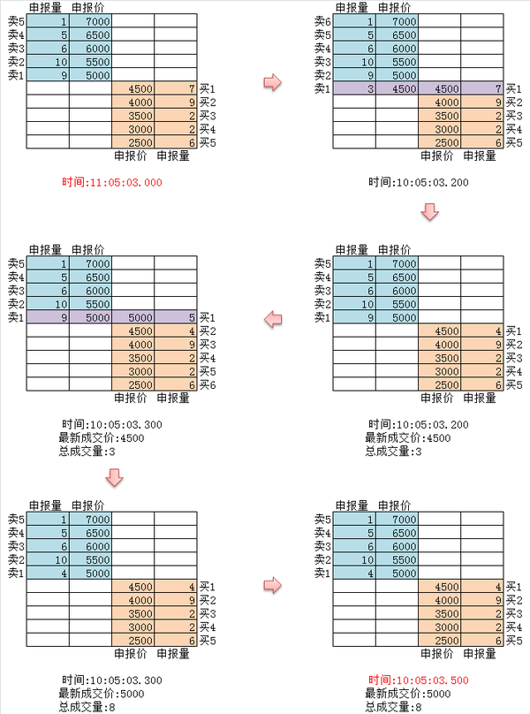
\includegraphics[width=1\textwidth]{figures/fig1.png}
      \end{figure}
    \column{5cm}
    \begin{figure}
      \centering
      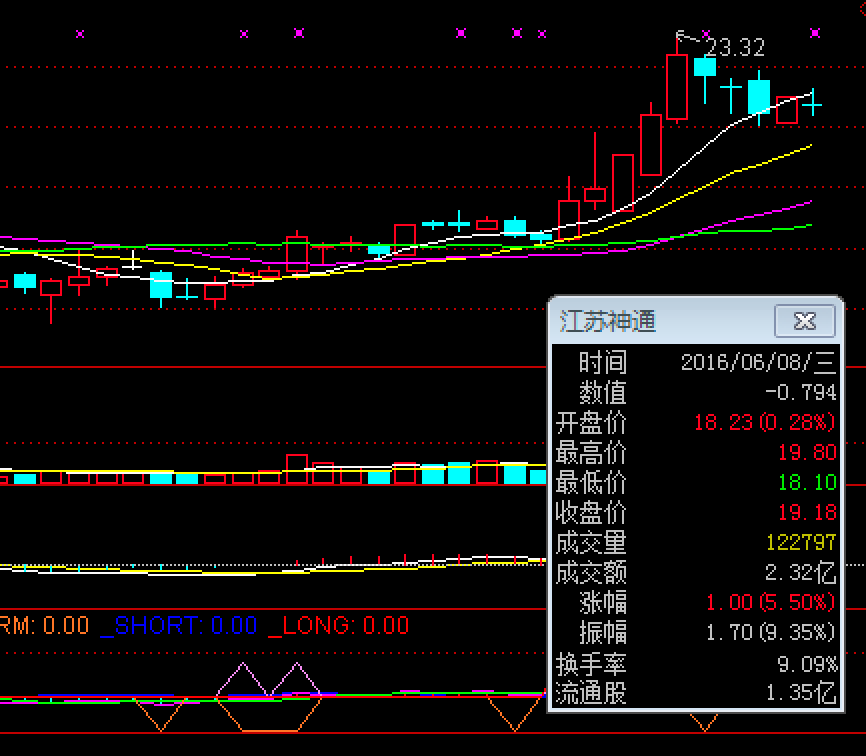
\includegraphics[width=1\textwidth]{figures/fig2.png}
      \end{figure}
  \end{columns}
  \end{frame}

\section{交易市场}

\begin{frame}{报价驱动市场}
\begin{table}
  \centering
  \begin{subtable}[b]{0.3\textwidth}
    \resizebox{\textwidth}{!}{
      \setlength{\arrayrulewidth}{2pt}
      \arrayrulecolor{orange}
      \begin{tabular}{>{\columncolor{mycyan}}c|>{\columncolor{mycyan}}c|>{\columncolor{mypink}}c|>{\columncolor{mypink}}c}
        \arrayrulecolor{orange}\hline
        \multicolumn{1}{>{\columncolor{cyan}}c|}{\color{white}\textsf{Offer Price}} &  \multicolumn{1}{>{\columncolor{cyan}}c}{\color{white}\textsf{Offer Quantity}}
        & \multicolumn{1}{>{\columncolor{pink}}c|}{\color{white}\textsf{Bid Price}} &  \multicolumn{1}{>{\columncolor{pink}}c}{\color{white}\textsf{Bid Quantity}}\\ 
        \arrayrulecolor{orange}\hline
         &  &  &  \\
        \arrayrulecolor{orange}\hline
        {100.0} & {1} & {} & {} \\
        \arrayrulecolor{orange}\hline
      \end{tabular}
    }
    \caption*{1}
  \end{subtable}
  \begin{subtable}[b]{0.3\textwidth}
    \resizebox{\textwidth}{!}{
      \setlength{\arrayrulewidth}{2pt}
      \arrayrulecolor{orange}
      \begin{tabular}{>{\columncolor{mycyan}}c|>{\columncolor{mycyan}}c|>{\columncolor{mypink}}c|>{\columncolor{mypink}}c}
        \arrayrulecolor{orange}\hline
        \multicolumn{1}{>{\columncolor{cyan}}c|}{\color{white}\textsf{Offer Price}} &  \multicolumn{1}{>{\columncolor{cyan}}c}{\color{white}\textsf{Offer Quantity}}
        & \multicolumn{1}{>{\columncolor{pink}}c|}{\color{white}\textsf{Bid Price}} &  \multicolumn{1}{>{\columncolor{pink}}c}{\color{white}\textsf{Bid Quantity}}\\ 
        \arrayrulecolor{orange}\hline
         &  &  & \\
        \arrayrulecolor{orange}\hline
        {100.0} & {1} & {98.0} & {2} \\
        \arrayrulecolor{orange}\hline
      \end{tabular}
    }
    \caption*{2}
  \end{subtable}
  \begin{subtable}[b]{0.3\textwidth}
    \resizebox{\textwidth}{!}{
      \setlength{\arrayrulewidth}{2pt}
      \arrayrulecolor{orange}
      \begin{tabular}{>{\columncolor{mycyan}}c|>{\columncolor{mycyan}}c|>{\columncolor{mypink}}c|>{\columncolor{mypink}}c}
        \arrayrulecolor{orange}\hline
        \multicolumn{1}{>{\columncolor{cyan}}c|}{\color{white}\textsf{Offer Price}} &  \multicolumn{1}{>{\columncolor{cyan}}c}{\color{white}\textsf{Offer Quantity}}
        & \multicolumn{1}{>{\columncolor{pink}}c|}{\color{white}\textsf{Bid Price}} &  \multicolumn{1}{>{\columncolor{pink}}c}{\color{white}\textsf{Bid Quantity}}\\ 
        \arrayrulecolor{orange}\hline
        102.0 & 2 &  & \\
        \arrayrulecolor{orange}\hline
        100.0 & 1 & 98.0&2 \\
        \arrayrulecolor{orange}\hline
      \end{tabular}
    }
    \caption*{3}
    \end{subtable}
\end{table}
\begin{table}
  \centering
  \begin{subtable}[b]{0.3\textwidth}
    \resizebox{\textwidth}{!}{
      \setlength{\arrayrulewidth}{2pt}
      \arrayrulecolor{orange}
      \begin{tabular}{>{\columncolor{mycyan}}c|>{\columncolor{mycyan}}c|>{\columncolor{mypink}}c|>{\columncolor{mypink}}c}
        \arrayrulecolor{orange}\hline
        \multicolumn{1}{>{\columncolor{cyan}}c|}{\color{white}\textsf{Offer Price}} &  \multicolumn{1}{>{\columncolor{cyan}}c}{\color{white}\textsf{Offer Quantity}}
        & \multicolumn{1}{>{\columncolor{pink}}c|}{\color{white}\textsf{Bid Price}} &  \multicolumn{1}{>{\columncolor{pink}}c}{\color{white}\textsf{Bid Quantity}}\\ 
        \arrayrulecolor{orange}\hline
        102.0 & 2 &  &  \\
        \arrayrulecolor{orange}\hline
        \sout{\textcolor{red}{100.0}} & \sout{\textcolor{red}{1}} & {98.0} & {2} \\
        \arrayrulecolor{orange}\hline
      \end{tabular}
    }
    \caption*{4}
  \end{subtable}
  \begin{subtable}[b]{0.3\textwidth}
    \resizebox{\textwidth}{!}{
      \setlength{\arrayrulewidth}{2pt}
      \arrayrulecolor{orange}
      \begin{tabular}{>{\columncolor{mycyan}}c|>{\columncolor{mycyan}}c|>{\columncolor{mypink}}c|>{\columncolor{mypink}}c}
        \arrayrulecolor{orange}\hline
        \multicolumn{1}{>{\columncolor{cyan}}c|}{\color{white}\textsf{Offer Price}} &  \multicolumn{1}{>{\columncolor{cyan}}c}{\color{white}\textsf{Offer Quantity}}
        & \multicolumn{1}{>{\columncolor{pink}}c|}{\color{white}\textsf{Bid Price}} &  \multicolumn{1}{>{\columncolor{pink}}c}{\color{white}\textsf{Bid Quantity}}\\ 
        \arrayrulecolor{orange}\hline
        102.0 & 2 & 98.0& 2 \\
        \arrayrulecolor{orange}\hline
        {} & {} & {} & {} \\
        \arrayrulecolor{orange}\hline
      \end{tabular}
    }
    \caption*{5}
  \end{subtable}
\end{table}
\end{frame}

\begin{frame}{坐市商市场}
  双方报价,点差比较大
  \begin{itemize}
    \item 典型:外汇市场,譬如银行的外汇兑换牌价
    \end{itemize}
\begin{table}
  \centering
  \begin{subtable}[b]{0.3\textwidth}
    \resizebox{\textwidth}{!}{
      \setlength{\arrayrulewidth}{2pt}
      \arrayrulecolor{orange}
      \begin{tabular}{>{\columncolor{mycyan}}c|>{\columncolor{mycyan}}c|>{\columncolor{mypink}}c|>{\columncolor{mypink}}c}
        \arrayrulecolor{orange}\hline
        \multicolumn{1}{>{\columncolor{cyan}}c|}{\color{white}\textsf{Offer Price}} &  \multicolumn{1}{>{\columncolor{cyan}}c}{\color{white}\textsf{Offer Quantity}}
        & \multicolumn{1}{>{\columncolor{pink}}c|}{\color{white}\textsf{Bid Price}} &  \multicolumn{1}{>{\columncolor{pink}}c}{\color{white}\textsf{Bid Quantity}}\\ 
        \arrayrulecolor{orange}\hline
        6.6200 &  $\ldots$&6.5600  & $\ldots$ \\
        \arrayrulecolor{orange}\hline
        &  &  &  \\
        \arrayrulecolor{orange}\hline
      \end{tabular}
    }
    \caption*{1}
  \end{subtable}
  \begin{subtable}[b]{0.3\textwidth}
    \resizebox{\textwidth}{!}{
    \setlength{\arrayrulewidth}{2pt}
      \arrayrulecolor{orange}
      \begin{tabular}{>{\columncolor{mycyan}}c|>{\columncolor{mycyan}}c|>{\columncolor{mypink}}c|>{\columncolor{mypink}}c}
        \arrayrulecolor{orange}\hline
        \multicolumn{1}{>{\columncolor{cyan}}c|}{\color{white}\textsf{Offer Price}} &  \multicolumn{1}{>{\columncolor{cyan}}c}{\color{white}\textsf{Offer Quantity}}
        & \multicolumn{1}{>{\columncolor{pink}}c|}{\color{white}\textsf{Bid Price}} &  \multicolumn{1}{>{\columncolor{pink}}c}{\color{white}\textsf{Bid Quantity}}\\ 
        \arrayrulecolor{orange}\hline
        6.6205 &  $\ldots$&6.5605  & $\ldots$ \\
        \arrayrulecolor{orange}\hline
        &  &  &  \\
        \arrayrulecolor{orange}\hline
      \end{tabular}
    }
    \caption*{2}
  \end{subtable}
\end{table}
\end{frame}

\begin{frame}{有坐市商报价驱动市场}
\begin{table}
  \centering
  \begin{subtable}[b]{0.3\textwidth}
    \resizebox{\textwidth}{!}{
      \setlength{\arrayrulewidth}{2pt}
      \arrayrulecolor{orange}
      \begin{tabular}{>{\columncolor{mycyan}}c|>{\columncolor{mycyan}}c|>{\columncolor{mypink}}c|>{\columncolor{mypink}}c}
        \arrayrulecolor{orange}\hline
        \multicolumn{1}{>{\columncolor{cyan}}c|}{\color{white}\textsf{Offer Price}} &  \multicolumn{1}{>{\columncolor{cyan}}c}{\color{white}\textsf{Offer Quantity}}
        & \multicolumn{1}{>{\columncolor{pink}}c|}{\color{white}\textsf{Bid Price}} &  \multicolumn{1}{>{\columncolor{pink}}c}{\color{white}\textsf{Bid Quantity}}\\ 
        \arrayrulecolor{orange}\hline
        98 &  10 & 92 & 10 \\
        \arrayrulecolor{orange}\hline
        &  &  &  \\
        \arrayrulecolor{orange}\hline
      \end{tabular}
    }
    \caption*{1}
  \end{subtable}
  \begin{subtable}[b]{0.3\textwidth}
    \resizebox{\textwidth}{!}{
    \setlength{\arrayrulewidth}{2pt}
      \arrayrulecolor{orange}
      \begin{tabular}{>{\columncolor{mycyan}}c|>{\columncolor{mycyan}}c|>{\columncolor{mypink}}c|>{\columncolor{mypink}}c}
        \arrayrulecolor{orange}\hline
        \multicolumn{1}{>{\columncolor{cyan}}c|}{\color{white}\textsf{Offer Price}} &  \multicolumn{1}{>{\columncolor{cyan}}c}{\color{white}\textsf{Offer Quantity}}
        & \multicolumn{1}{>{\columncolor{pink}}c|}{\color{white}\textsf{Bid Price}} &  \multicolumn{1}{>{\columncolor{pink}}c}{\color{white}\textsf{Bid Quantity}}\\ 
        \arrayrulecolor{orange}\hline
        98 & \textcolor{red}{10-2} & \sout{\textcolor{red}{98}}& \sout{\textcolor{red}{2}} \\
        \arrayrulecolor{orange}\hline
        &  & 92 & 10 \\
        \arrayrulecolor{orange}\hline
      \end{tabular}
    }
    \caption*{2}
  \end{subtable}
\end{table}
\begin{table}
\resizebox{0.4\textwidth}{!}{
    \setlength{\arrayrulewidth}{2pt}
      \arrayrulecolor{orange}
      \begin{tabular}{>{\columncolor{mycyan}}c|>{\columncolor{mycyan}}c|>{\columncolor{mypink}}c|>{\columncolor{mypink}}c}
        \arrayrulecolor{orange}\hline
        \multicolumn{1}{>{\columncolor{cyan}}c|}{\color{white}\textsf{Offer Price}} &  \multicolumn{1}{>{\columncolor{cyan}}c}{\color{white}\textsf{Offer Quantity}}
        & \multicolumn{1}{>{\columncolor{pink}}c|}{\color{white}\textsf{Bid Price}} &  \multicolumn{1}{>{\columncolor{pink}}c}{\color{white}\textsf{Bid Quantity}}\\ 
        \arrayrulecolor{orange}\hline
        98 & 10 & \textcolor{red}{93}& \textcolor{red}{2} \\
        \arrayrulecolor{orange}\hline
        &  & 92 & 10 \\
        \arrayrulecolor{orange}\hline
      \end{tabular}
    }
    \caption*{3}
\end{table}
\end{frame}

\end{document}
